\begin{refsection} % refsection environment
\chapter[Short title]{Long title}


\addcontentsline{toc}{section}{References}
\printbibliography[heading=subbibliography, title={References}] % print section bibliography

\begin{appendices}
	\chapter{Appendix I}
	This is a reference \cite{Al_Amin_1996}.
	
	This is a table. 
	
	\begin{table}[h!]
		\centering
		\begin{tabular}{||c c c c||} 
			\hline
			Col1 & Col2 & Col2 & Col3 \\ [0.5ex] 
			\hline\hline
			1 & 6 & 87837 & 787 \\ 
			2 & 7 & 78 & 5415 \\
			3 & 545 & 778 & 7507 \\
			4 & 545 & 18744 & 7560 \\
			5 & 88 & 788 & 6344 \\ [1ex] 
			\hline
		\end{tabular}
		\caption{Table to test captions and labels}
		\label{table:3}
	\end{table}

	This is a figure.
	
	\begin{figure}[ht]
		\centering
		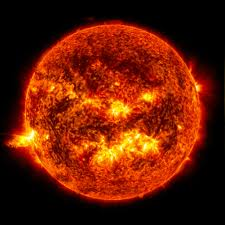
\includegraphics[]{sun}
		\caption[The sun]{The Sun is the star at the center of the Solar System.}
		\centering
		\label{fig:2}
	\end{figure}
	

	
	\chapter{Appendix II}
\end{appendices}

\end{refsection}